\chapter{Electromagnetic Induction and Applications}\label{ch:b1:induction}

Move a magnet toward a coil and a current flows in the coil; stop the
magnet and the current stops. Faraday found this in 1831, after ten
years of looking, and it is the fact on which the electrical world
runs: every power station, every transformer, every motor and
loudspeaker and microphone, every induction cooktop and wireless
charger converts energy through the law that a \emph{changing} \omterm{def:b1:induction:flux}{magnetic
flux} drives an \omterm{def:b1:dc-circuits:sources}{electromotive force}. This chapter states the law with
its signs, gives it the two faces it wears (a changing field in a fixed
circuit, a circuit moving in a fixed field), defines self and \omterm{def:b1:induction:inductance}{mutual
inductance}, and then works through the electromechanical machines ---
the sliding bar, the alternator, the transformer, the loudspeaker ---
where the same law turns mechanical power into electrical power and
back, never for free.

\begin{omfigure}
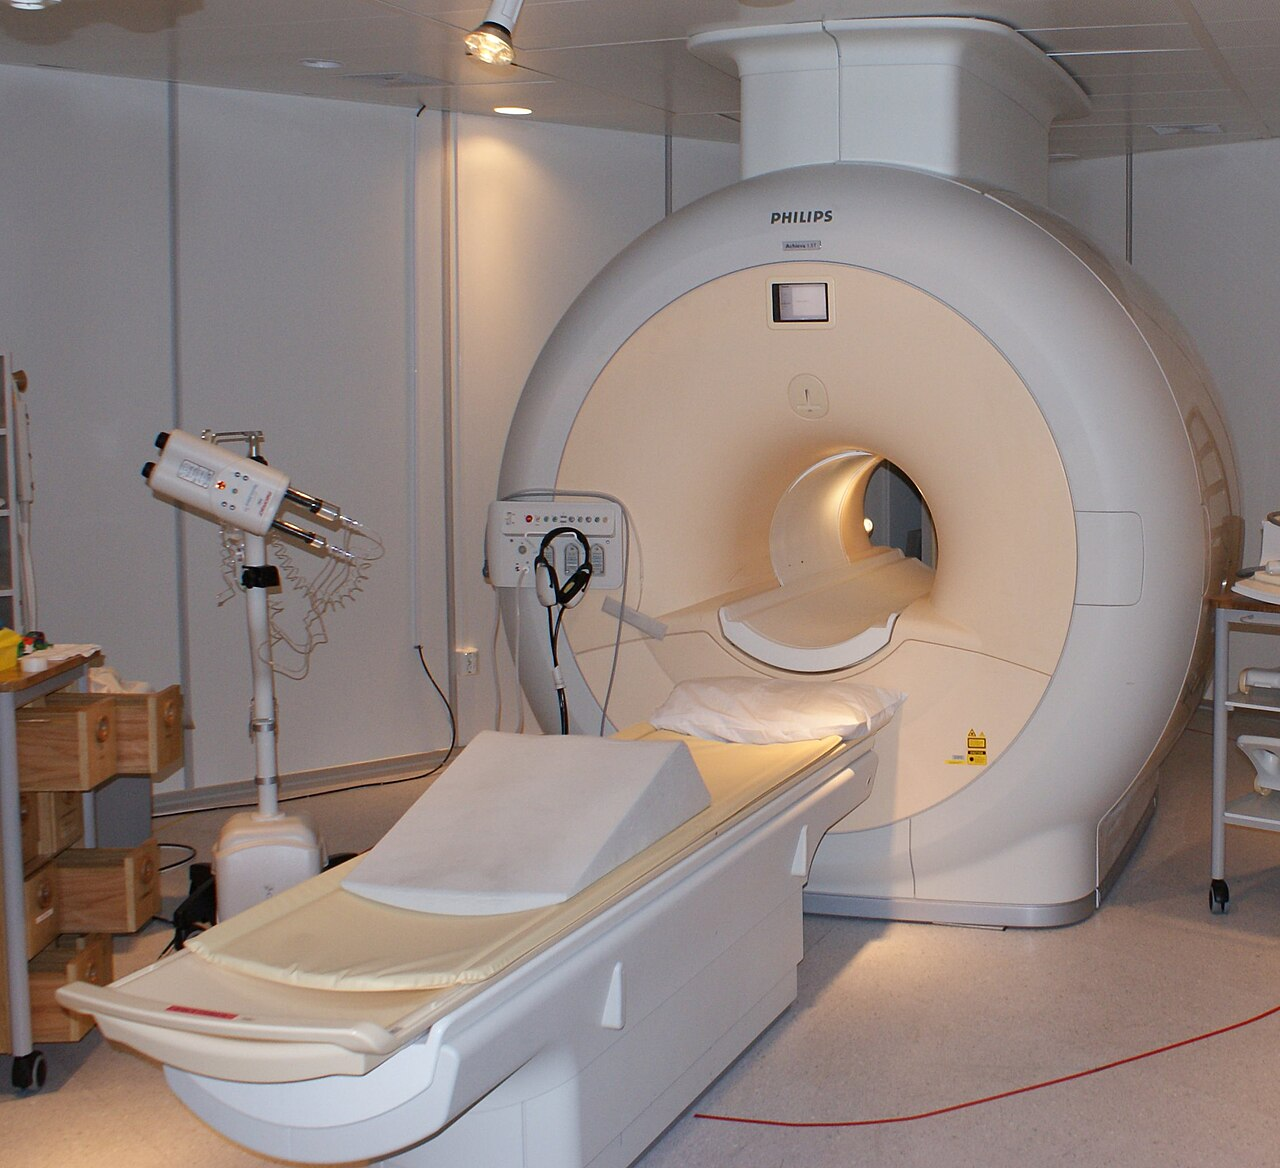
\includegraphics[width=0.50\linewidth]{images/book3/mri-scanner.jpg}

{\small An MRI scanner: a superconducting solenoid holding \qty{1.5}{T} over a patient --- a megajoule of \omterm{prop:b1:induction:inductor}{magnetic energy} in a field with nothing in it. Photograph: Jan Ainali, CC~BY~3.0.}
\end{omfigure}

\section{Faraday's law}

\begin{definition}[Magnetic flux through a circuit]\label{def:b1:induction:flux}
\index{magnetic flux}\index{weber}
Orient a closed circuit $\Gamma$ (a sense of travel); its surface gets
the normal $\vect n$ given by the right-hand rule. The \emph{magnetic
flux} through the circuit is $\Phi = \sum\vect B\cdot\vect n\,\dd S$ over
any surface bounded by $\Gamma$ (weber, $\qty{1}{Wb} = \qty{1}{T.m^2}$) ---
``any'', because the flux of $\vect B$ through a closed surface is zero.
For a uniform field and a plane coil of $N$ turns and area $S$, $\Phi =
NBS\cos\alpha$, $\alpha$ the angle between $\vect B$ and $\vect n$.
\end{definition}

\begin{theorem}[Faraday's law of induction]\label{thm:b1:induction:faraday}
\index{Faraday's law}\index{electromotive force (induced)}\index{Lenz's law}
Whenever the flux through a circuit varies, the circuit is the seat of
an \emph{induced \omterm{def:b1:dc-circuits:sources}{electromotive force}}
\[
e = -\frac{\dd\Phi}{\dd t} ,
\]
counted in the orientation of the circuit, i.e.\ acting as an ideal
\omterm{def:b1:dc-circuits:sources}{voltage source} of emf $e$ in that sense; in a circuit of resistance $R$
it drives the current $i = e/R$. The minus sign is \emph{\omterm{thm:b1:induction:faraday}{Lenz's law}}:
the induced current flows so as to oppose the change of flux that
produces it --- its own field, and the forces it feels, fight the cause.
\end{theorem}
\admitted

\begin{remark}[Two faces of the same law]\label{rem:b1:induction:twofaces}
\index{Neumann induction}\index{Lorentz induction}
The flux changes either because $\vect B$ varies in time through a
fixed circuit (\emph{\omterm{rem:b1:induction:twofaces}{Neumann induction}}: transformer, induction cooktop)
or because the circuit moves or deforms in a steady field
(\emph{\omterm{rem:b1:induction:twofaces}{Lorentz induction}}: generator, loudspeaker). In the second case
the emf can also be computed directly: the carriers of a conductor
element $\dd\vect l$ moving at $\vect v$ feel the force $q\vect v\wedge
\vect B$, equivalent to an electric field $\vect v\wedge\vect B$, so that
$e = \oint(\vect v\wedge\vect B)\cdot\dd\vect l$ --- and this always agrees
with $-\dd\Phi/\dd t$. \omterm{thm:b1:induction:faraday}{Faraday's law} covers both; the Year 2 volume
explains why the two mechanisms give one formula.
\end{remark}

\begin{omfigure}
\begin{tikzpicture}[font=\small, x=1cm, y=1cm, >=Stealth]
  \begin{scope}
    \draw[omThm, very thick, postaction={decorate, decoration={markings, mark=at position 0.25 with {\arrow{>}}, mark=at position 0.75 with {\arrow{>}}}}] (0,0) ellipse (1.4 and 0.5);
    \draw[omDef, thick, ->] (0,0.5) -- (0,1.7) node[right, font=\footnotesize] {$\vect n$};
    \node[omThm, font=\footnotesize] at (1.75,-0.55) {$\Gamma$};
    \foreach \x in {-0.9,-0.3,0.3,0.9} \draw[omProp, ->] (\x,-1.6) -- (\x,1.2);
    \node[omProp, font=\footnotesize] at (1.4,1.05) {$\vect B$};
    \node[font=\footnotesize] at (0,-2.2) {$\Phi = \vect B\cdot\vect n\,S > 0$};
  \end{scope}
  \begin{scope}[xshift=6.2cm]
    \draw[omThm, very thick, postaction={decorate, decoration={markings, mark=at position 0.25 with {\arrow{<}}, mark=at position 0.75 with {\arrow{<}}}}] (0,0) ellipse (1.4 and 0.5);
    \node[omThm, font=\footnotesize] at (1.75,0.6) {$i$};
    % magnet coming down
    \draw[fill=omDef!20, draw=omDef, thick] (-0.4,1.3) rectangle (0.4,2.0); \node[omDef, font=\footnotesize] at (0,1.65) {S};
    \draw[fill=omThm!20, draw=omThm, thick] (-0.4,2.0) rectangle (0.4,2.7); \node[omThm, font=\footnotesize] at (0,2.35) {N};
    \draw[very thick, ->] (0.8,2.6) -- (0.8,1.7) node[right, font=\footnotesize] {$\vect v$};
    \draw[omProp, ->] (0,1.25) -- (0,0.2) node[right, font=\footnotesize, pos=0.6] {$\vect B$ (magnet)};
    \draw[omDef, ->] (-0.6,-0.1) -- (-0.6,0.9) node[left, font=\footnotesize, pos=0.7] {$\vect B_{\text{ind}}$};
    \node[font=\footnotesize] at (0,-2.2) {approaching magnet: $i$ repels it};
  \end{scope}
  \begin{scope}[xshift=11.8cm]
    \draw[omThm, very thick] (-1.4,-0.5) rectangle (1.4,0.5);
    \draw[omThm, very thick] (0.5,-0.5) -- (0.5,0.5);
    \draw[omDef, very thick, ->] (0.5,0.5) -- (0.5,-0.5);
    \draw[very thick, ->] (0.6,0.75) -- (1.2,0.75) node[above, font=\footnotesize] {$\vect v$};
    \foreach \x in {-1.1,-0.6,-0.1,0.4,0.9} \node[omProp, font=\scriptsize] at (\x,0.0) {$\odot$};
    \node[omProp, font=\footnotesize] at (1.75,0.0) {$\vect B$};
    \draw[omDef, ->, thick] (0.5,0.0) -- (-0.2,0.0); \node[omDef, font=\footnotesize] at (-0.15,-0.3) {$\vect F$};
    \node[font=\footnotesize] at (0,-2.2) {sliding bar: flux grows, $\vect F$ brakes};
  \end{scope}
\end{tikzpicture}

{\small Orientation and \omterm{thm:b1:induction:faraday}{Lenz's law}. Left: the circuit's orientation
fixes $\vect n$ and the sign of $\Phi$. Middle: a magnet approaching a
ring increases the flux; the induced current creates a field opposing
the magnet's and the ring repels it. Right: a bar sliding on rails in a
field pointing toward the reader; the flux of the circuit grows, the
induced current flows so that the \omterm{thm:b1:magnetostatics:laplace}{Laplace force} on the bar opposes its
motion.}
\end{omfigure}

\begin{example}[Orders of magnitude]\label{ex:b1:induction:orders}
A coil of $100$ turns and \qty{10}{cm^2} in the Earth's field, flipped in
\qty{0.1}{s}: $\Delta\Phi = 2 \times 100 \times 10^{-3} \times 5 \times 10^{-5} = \qty{1e-5}{Wb}$,
$e \sim \qty{0.1}{mV}$ --- measurable with a sensitive galvanometer, the way
the Earth's field was once mapped. The same coil in the \qty{1}{T} gap
of a magnet, pulled out in \qty{0.1}{s}: \qty{1}{V}. A transformer coil of
$1000$ turns with \qty{1}{T} at \qty{50}{Hz} over \qty{10}{cm^2}: $e_{\max} =
1000 \times 10^{-3} \times 314 = \qty{314}{V}$ --- the mains.
\end{example}

\section{Self and mutual inductance}

\begin{definition}[Inductance]\label{def:b1:induction:inductance}
\index{self-inductance}\index{henry}\index{mutual inductance}
The flux of a circuit's own field through itself is proportional to its
current: $\Phi_{\text{own}} = Li$, with $L > 0$ its \emph{self-inductance}
(henry, \unit{H}). The flux that circuit~1 sends through circuit~2 is
$\Phi_{1 \to 2} = Mi_1$, and symmetrically $\Phi_{2 \to 1} = Mi_2$, with $M$
their \emph{mutual inductance} (sign fixed by the orientations). The
total flux of circuit~1 is then $\Phi_1 = L_1i_1 + Mi_2$.
\end{definition}

\begin{proposition}[The inductor; the solenoid]\label{prop:b1:induction:inductor}
\index{inductor}\index{magnetic energy}\index{energy density of the magnetic field}
A circuit of inductance $L$ carrying a varying current is the seat of
the emf $e = -L\,\dd i/\dd t$: in the \omterm{thm:b1:dc-circuits:kirchhoff}{receiver convention} this is the
\omterm{def:b1:dc-circuits:voltage}{voltage} $u = L\,\dd i/\dd t$ of the inductor used since
\cref{ch:b1:transient-regimes}. It stores the energy $W = \tfrac12Li^2$.
A long solenoid of $n$ turns per metre, length $\ell$, section $S$,
has $L = \mu_0n^2S\ell$; its stored energy is $\tfrac12\mu_0n^2I^2S\ell =
\dfrac{B^2}{2\mu_0}\,S\ell$: \omterm{prop:b1:induction:inductor}{magnetic energy} lives in the field at the
density $B^2/2\mu_0$, exactly as electric energy at $\varepsilon_0E^2/2$.
\end{proposition}

\begin{proof}
Faraday with $\Phi = Li$, $L$ constant. Energy: the power received by
the inductor is $ui = Li\,\dd i/\dd t = \dd(\tfrac12Li^2)/\dd t$. Solenoid:
$B = \mu_0nI$ inside, flux $BS$ through each of the $n\ell$ turns, so $\Phi =
\mu_0n^2S\ell I$. The general density is admitted.
\end{proof}

\begin{example}[An MRI magnet]\label{ex:b1:induction:mri}
\qty{1.5}{T} over about a cubic metre: $B^2/2\mu_0 = 2.25/2.5 \times 10^{-6} =
\qty{0.9}{MJ/m^3}$ --- the energy of a car battery, stored in empty space.
With a coil current of \qty{500}{A}, $L = 2W/I^2 = \qty{7}{H}$. If the
superconductor suddenly turns resistive (a \emph{quench}), that megajoule
becomes heat in seconds and boils off hundreds of litres of liquid
helium: the magnet room has a vent for it.
\end{example}

\begin{proposition}[The ideal transformer]\label{prop:b1:induction:transformer}
\index{transformer}
Two coils of $N_1$ and $N_2$ turns wound on the same closed iron core,
so that the same flux $\varphi$ threads every turn, obey
\[
\frac{u_2}{u_1} = \frac{N_2}{N_1} , \qquad N_1i_1 + N_2i_2 = 0 \quad\text{(no load losses, no magnetizing current)},
\]
so that $u_2i_2 = -u_1i_1$: the power taken at the primary is delivered
at the secondary; \omterm{def:b1:dc-circuits:voltage}{voltages} step with the turns ratio, currents
inversely. It works only with varying currents.
\end{proposition}

\begin{proof}
$u_1 = N_1\,\dd\varphi/\dd t$ and $u_2 = N_2\,\dd\varphi/\dd t$ (\omterm{thm:b1:dc-circuits:kirchhoff}{receiver
convention} on both, orientations chosen along the common flux): divide.
The current relation is \omterm{thm:b1:magnetostatics:ampere}{Ampère's law} on the core: its circulation
$\mu_0\mu_r$-times the total ampere-turns would have to create the
flux; for an ideal core ($\mu_r \to \infty$) that takes vanishing
ampere-turns, hence $N_1i_1 + N_2i_2 = 0$. Admitted in this form.
\end{proof}

\begin{omfigure}
\begin{tikzpicture}[font=\small, x=1cm, y=1cm, >=Stealth]
  % core
  \draw[omExo!60, line width=9pt] (-2,-1.5) rectangle (2,1.5);
  % primary windings
  \foreach \y in {-0.9,-0.6,...,0.9} \draw[omThm, thick] (-2.35,\y) arc[start angle=90, end angle=-90, x radius=0.18, y radius=0.15];
  \foreach \y in {-0.9,-0.6,...,0.9} \draw[omDef, thick] (2.35,\y) arc[start angle=90, end angle=270, x radius=0.18, y radius=0.15];
  \draw[omThm, thick] (-2.35,0.9) -- (-3.2,0.9) node[left, font=\footnotesize] {$u_1$}; \draw[omThm, thick] (-2.35,-1.2) -- (-3.2,-1.2);
  \draw[omDef, thick] (2.35,0.9) -- (3.2,0.9) node[right, font=\footnotesize] {$u_2$}; \draw[omDef, thick] (2.35,-1.2) -- (3.2,-1.2);
  \node[omThm, font=\footnotesize] at (-2.9,0) {$N_1$}; \node[omDef, font=\footnotesize] at (2.9,0) {$N_2$};
  \draw[omProp, thick, dashed, ->] (-1.3,-0.9) -- (-1.3,0.9) -- (1.3,0.9) -- (1.3,-0.9) -- cycle;
  \node[omProp, font=\footnotesize] at (0,0) {flux $\varphi$};
  \node[font=\footnotesize] at (0,-2.2) {$u_2/u_1 = N_2/N_1$, \quad $N_1 i_1 = -N_2 i_2$};
  \begin{scope}[xshift=8.6cm]
    \draw[omThm, very thick] (-1.6,0) -- (1.6,0);
    \foreach \x in {-1.3,-0.9,...,1.3} \draw[omThm, thick] (\x,0) arc[start angle=180, end angle=0, x radius=0.2, y radius=0.45];
    \draw[omDef, very thick] (-1.2,-1.1) -- (1.2,-1.1);
    \foreach \x in {-0.9,-0.5,...,0.9} \draw[omDef, thick] (\x,-1.1) arc[start angle=180, end angle=0, x radius=0.2, y radius=0.35];
    \node[omThm, font=\footnotesize] at (-2.1,0.3) {$i_1$, $L_1$}; \node[omDef, font=\footnotesize] at (-1.9,-0.9) {$L_2$};
    \draw[<->, omProp] (0,0.7) -- (0,-0.9) node[midway, right, font=\footnotesize] {$M$};
    \node[font=\footnotesize] at (0,-2.2) {$\Phi_1 = L_1 i_1 + M i_2$};
  \end{scope}
\end{tikzpicture}

{\small Left: a transformer --- two coils on a closed iron core share
the same flux; the \omterm{def:b1:dc-circuits:voltage}{voltages} scale with the turns, the currents
inversely. Right: two coupled coils in air and their \omterm{def:b1:induction:inductance}{mutual
inductance} $M$; a coil's own flux is $Li$.}
\end{omfigure}

\section{Moving conductors: generators and motors}

\begin{proposition}[The sliding bar]\label{prop:b1:induction:rails}
\index{Laplace rails}\index{electromechanical conversion}
A bar of length $\ell$ slides at speed $v$ on two rails closed by a
resistance $R$, in a uniform field $B$ normal to the plane. It is the
seat of the emf $e = B\ell v$, drives $i = B\ell v/R$, and feels the
\omterm{thm:b1:magnetostatics:laplace}{Laplace force} $F = B\ell i = B^2\ell^2v/R$ \emph{opposing} its motion.
The mechanical power spent to push it, $Fv$, equals the electrical
power $ei = Ri^2$ dissipated: the bar is a generator. Fed instead by a
source $E$, it is a motor: the current $(E - B\ell v)/R$ pushes it
until the back-emf $B\ell v$ balances $E$, at the no-load speed $E/B\ell$.
\end{proposition}

\begin{proof}
Flux $B\ell x$, $e = -B\ell\dot x$ in the orientation for which $\vect n$ is
along $\vect B$; the \omterm{thm:b1:magnetostatics:laplace}{Laplace force} $i\vect\ell\wedge\vect B$ on the current
so oriented points against $\vect v$ (\cref{thm:b1:induction:faraday},
Lenz). Multiply the electrical equation $e = Ri$ by $i$ and the
mechanical one by $v$: $Fv = B\ell iv = ei$. The electromechanical
power $ei$ and the Laplace power $-Fv$ are always opposite --- the law
of the conversion.
\end{proof}

\begin{proposition}[The rotating loop: alternator]\label{prop:b1:induction:alternator}
\index{alternator}
A coil of $N$ turns and area $S$ rotating at $\omega$ about an axis
perpendicular to a uniform $B$ has $\Phi = NBS\cos\omega t$ and
\[
e = NBS\omega\sin\omega t :
\]
a sinusoidal emf of \omterm{def:b1:wave-propagation:signal}{amplitude} $NBS\omega$ and the frequency of rotation.
Into a resistance $R$ it delivers the mean power $(NBS\omega)^2/2R$,
supplied by the \omterm{def:b1:angular-momentum:moment}{torque} that keeps it turning against the Laplace
couple $-\vect m\wedge\vect B$ of its own current.
\end{proposition}

\begin{proof}
Differentiate the flux; $\langle\sin^2\rangle = \tfrac12$. The couple is
\cref{thm:b1:magnetostatics:dipoleinfield} with $m = Ni S$; its mean
power $\langle\Gamma\omega\rangle$ equals $\langle ei\rangle$ by the same
computation as for the bar.
\end{proof}

\begin{omfigure}
\begin{tikzpicture}[font=\small, x=1cm, y=1cm, >=Stealth]
  \begin{scope}
    \draw[omThm, very thick] (-1.8,-1.0) -- (1.8,-1.0); \draw[omThm, very thick] (-1.8,1.0) -- (1.8,1.0);
    \draw[omThm, very thick] (-1.8,-1.0) -- (-1.8,1.0);
    \draw[omDef, very thick] (0.8,-1.0) -- (0.8,1.0);
    \draw[omDef, very thick, ->] (0.8,-0.2) -- (0.8,0.3) node[right, font=\footnotesize] {$i$};
    \draw[omProp, thick, ->] (0.8,0) -- (0.05,0) node[above, font=\footnotesize, pos=0.5] {$\vect F$};
    \draw[very thick, ->] (1.0,1.25) -- (1.7,1.25) node[right, font=\footnotesize] {$\vect v$};
    \foreach \x in {-1.4,-0.9,-0.4,0.1,1.3} \foreach \y in {-0.5,0.5} \node[omProp, font=\scriptsize] at (\x,\y) {$\odot$};
    \draw[fill=white] (-1.95,-0.35) rectangle (-1.65,0.35); \node[font=\footnotesize] at (-2.45,0) {$R$};
    \node[font=\footnotesize] at (0,-1.6) {$e = B\ell v$, \; $F = B^2\ell^2 v/R$};
  \end{scope}
  \begin{scope}[xshift=6.5cm]
    \draw[omThm, very thick, rotate=30] (-1.2,-0.6) rectangle (1.2,0.6);
    \draw[dashed] (0,-1.6) -- (0,1.6); \node[font=\footnotesize] at (0,1.85) {axis};
    \foreach \y in {-1.2,-0.6,0,0.6,1.2} \draw[omProp, ->] (-2.2,\y) -- (2.2,\y);
    \node[omProp, font=\footnotesize] at (2.0,1.45) {$\vect B$};
    \draw[->, very thick] (0,0) -- (120:1.0) node[above left, font=\footnotesize] {$\vect n$};
    \draw (0.6,0) arc[start angle=0, end angle=120, radius=0.6] node[midway, above right, font=\footnotesize] {$\omega t$};
    \node[font=\footnotesize] at (0,-2.0) {$\Phi = NBS\cos\omega t$, \; $e = NBS\omega\sin\omega t$};
  \end{scope}
\end{tikzpicture}\hfill
\begin{tikzpicture}
\begin{axis}[omaxis, axis x line=middle, axis y line=left, width=4.3cm, height=3.8cm,
    xlabel={$t$}, ylabel={$e$}, xmin=0, xmax=6.6, ymin=-1.3, ymax=1.3, xtick=\empty, ytick=\empty, samples=80,
    xlabel style={at={(axis description cs:1.0,0.55)}, anchor=west}]
  \addplot[omDef, thick, domain=0:6.28] {sin(deg(x))};
\end{axis}
\end{tikzpicture}

{\small Left: the sliding bar as a generator --- emf $B\ell v$, current
through $R$, \omterm{thm:b1:magnetostatics:laplace}{Laplace force} braking the bar; the pusher's power is the
\omterm{def:b1:dc-circuits:resistor}{resistor}'s heat. Middle and right: the rotating coil of an alternator
and its sinusoidal emf.}
\end{omfigure}

\begin{example}[Eddy currents]\label{ex:b1:induction:eddy}
\index{eddy currents}
A bulk conductor moving in a non-uniform field, or sitting in a
varying one, is threaded by changing flux along countless closed paths:
\emph{\omterm{ex:b1:induction:eddy}{eddy currents}} circulate in it, heating it and --- by Lenz ---
braking it. A magnet dropped down a copper tube drifts down slowly; the
brakes of trucks and roller coasters use it (no contact, no wear, no
brake failure --- but no braking at rest); the induction cooktop heats
the pan by the same currents, at \qty{25}{kHz}; transformer cores are
laminated precisely to cut them.
\end{example}

\section{The loudspeaker: a coupled system}

\begin{proposition}[Electromechanical coupling of a coil in a radial field]\label{prop:b1:induction:loudspeaker}
\index{loudspeaker}\index{microphone}
A coil of total wire length $\ell$ sits in a radial field $B$ so that
every element of wire is perpendicular to $\vect B$; it moves along its
axis at speed $v$ and carries $i$. Then it feels the axial \omterm{thm:b1:magnetostatics:laplace}{Laplace force}
$F = B\ell i$ and is the seat of the back-emf $e = -B\ell v$ (\omterm{thm:b1:dc-circuits:kirchhoff}{receiver
convention}: a \omterm{def:b1:dc-circuits:voltage}{voltage} $B\ell v$). With a mass $m$, a suspension of
stiffness $k$ and a mechanical damping $h$, fed by a \omterm{def:b1:dc-circuits:voltage}{voltage} $u$ through
the coil's resistance $R$ and inductance $L$:
\[
u = Ri + L\frac{\dd i}{\dd t} + B\ell v , \qquad
m\frac{\dd v}{\dd t} = -kx - hv + B\ell i .
\]
Multiplying by $i$ and by $v$ and adding: the electrical power $ui$
equals the Joule loss $Ri^2$ plus the growth of the stored energies
$\tfrac12Li^2 + \tfrac12mv^2 + \tfrac12kx^2$ plus the mechanical loss
$hv^2$ (which includes the sound): the conversion term $B\ell iv$ cancels
between the two equations. Run backward (motion imposed, $u$ read) the
same device is a dynamic \emph{microphone}.
\end{proposition}

\begin{proof}
\omterm{thm:b1:magnetostatics:laplace}{Laplace force} on each element $i\,\dd\vect l\wedge\vect B$, all axial and
of the same sign; emf from $(\vect v\wedge\vect B)\cdot\dd\vect l$ summed
over the wire. The energy balance is the sum of the two equations
multiplied as stated.
\end{proof}

\begin{omfigure}
\begin{tikzpicture}[font=\small, x=1cm, y=1cm, >=Stealth]
  % magnet structure (cross-section)
  \draw[fill=omExo!30, draw=omExo, thick] (-3.0,-1.2) rectangle (-0.6,1.2);
  \draw[fill=omExo!30, draw=omExo, thick] (-0.6,-0.35) rectangle (1.6,0.35);
  \draw[fill=omExo!30, draw=omExo, thick] (-0.6,0.85) rectangle (1.6,1.2);
  \draw[fill=omExo!30, draw=omExo, thick] (-0.6,-1.2) rectangle (1.6,-0.85);
  \node[omExo, font=\footnotesize] at (-1.8,0) {magnet};
  % coil in the gaps
  \foreach \x in {0.9,1.05,1.2,1.35} {\fill[omThm] (\x,0.6) circle (1.6pt); \fill[omThm] (\x,-0.6) circle (1.6pt);}
  \node[omThm, font=\footnotesize] at (1.1,1.55) {voice coil};
  % radial field arrows in the gaps
  \foreach \x in {0.3,0.55} {\draw[omProp, ->] (\x,0.4) -- (\x,0.8); \draw[omProp, ->] (\x,-0.4) -- (\x,-0.8);}
  \node[omProp, font=\footnotesize] at (-0.2,0.6) {$\vect B$};
  % cone
  \draw[thick] (1.6,0.6) -- (3.4,2.2); \draw[thick] (1.6,-0.6) -- (3.4,-2.2);
  \draw[thick] (1.6,0.6) -- (1.6,-0.6);
  \node[font=\footnotesize] at (2.9,-0.95) {cone, $m$};
  \draw[thick, decorate, decoration={coil, aspect=0.6, segment length=3pt, amplitude=2pt}] (3.4,2.2) -- (3.4,2.9); \draw[thick] (3.0,2.9) -- (3.8,2.9);
  \draw[thick, decorate, decoration={coil, aspect=0.6, segment length=3pt, amplitude=2pt}] (3.4,-2.2) -- (3.4,-2.9); \draw[thick] (3.0,-2.9) -- (3.8,-2.9);
  \node[font=\footnotesize] at (3.4,3.25) {suspension $k$, $h$};
  \draw[omDef, very thick, ->] (1.6,0) -- (2.6,0);
  \node[omDef, font=\footnotesize, anchor=south west] at (1.75,0.08) {$F = B\ell i$};
  \draw[very thick, ->] (4.6,0.5) -- (5.6,0.5) node[right, font=\footnotesize] {$v$};
  \node[font=\footnotesize] at (5.3,-1.7) {$u = Ri + L\frac{\dd i}{\dd t} + B\ell v$};
\end{tikzpicture}

{\small A moving-coil loudspeaker in section: the voice coil sits in
the annular gap of a magnet where the field is radial, so that a
current gives an axial force whatever the position; the cone it drives
is held by a stiff, damped suspension; the coil's motion feeds a
back-emf $B\ell v$ into the electrical circuit.}
\end{omfigure}

\begin{remark}[Why the coupling damps]\label{rem:b1:induction:damping}
At low frequency ($L\omega \ll R$), $i \approx (u - B\ell v)/R$ and the force
is $B\ell u/R - (B^2\ell^2/R)\,v$: the electrical circuit adds the damping
$B^2\ell^2/R$ to the mechanical one. A loudspeaker connected to an
amplifier (low output resistance) is heavily damped --- its cone stops
when the \omterm{def:b1:wave-propagation:signal}{signal} stops --- and the same coupling is what lets the
microphone take energy from the sound (\cref{pb:b1:induction:1}).
\end{remark}

\section{Exercises}

\begin{exercise}[$\star$]\label{exo:b1:induction:1}
A coil of $100$ turns and \qty{10}{cm^2} in a uniform \qty{0.20}{T} field at
\qty{30}{\degree} to its normal. Flux; mean emf if the field is switched
off in \qty{10}{ms}; in \qty{1}{ms}; sense of the induced current
relative to the field (Lenz).
\end{exercise}

\begin{exercise}[$\star$]\label{exo:b1:induction:2}
A bar \qty{20}{cm} long slides at \qty{2.0}{m/s} on rails closed by
\qty{0.10}{\ohm}, in \qty{0.50}{T}. Emf, current, \omterm{thm:b1:magnetostatics:laplace}{Laplace force}, force the
pusher must apply, mechanical power, electrical power.
\end{exercise}

\begin{exercise}[$\star$]\label{exo:b1:induction:3}
Solenoid of \qty{1000}{turns/m}, length \qty{20}{cm}, section \qty{4.0}{cm^2}:
inductance; energy at \qty{5.0}{A}; \omterm{def:b1:transient-regimes:firstorder}{time constant} with a \qty{1.0}{\ohm}
resistance; field inside and energy density, to check $B^2/2\mu_0$.
\end{exercise}

\begin{exercise}[$\star$]\label{exo:b1:induction:4}
A transformer from \qty{230}{V} to \qty{12}{V}: turns ratio; primary
turns for a $50$-turn secondary; primary current when the secondary
delivers \qty{2.0}{A}. Why does it not work on a car battery?
\end{exercise}

\begin{exercise}[$\star\star$]\label{exo:b1:induction:5}
\omterm{thm:b1:induction:faraday}{Lenz's law}: give the sense of the induced current and the direction of
the force in each case --- (a) a north pole approaches a ring along
its axis; (b) a ring lies in a field that grows; (c) a ring is dropped
onto a magnet; (d) a magnet falls through a long copper tube. For (d),
explain with energy why it falls at a small constant speed.
\end{exercise}

\begin{exercise}[$\star\star$]\label{exo:b1:induction:6}
Alternator: $N = 200$, $S = \qty{20}{cm^2}$, $B = \qty{0.10}{T}$, \qty{50}{Hz}.
Peak and rms emf; peak current and peak \omterm{def:b1:angular-momentum:moment}{torque} into \qty{10}{\ohm}; mean
electrical power; compare with the mean mechanical power, and with the
instantaneous \omterm{def:b1:angular-momentum:moment}{torque} at the moment the emf vanishes.
\end{exercise}

\begin{exercise}[$\star\star$]\label{exo:b1:induction:7}
\emph{Magnetic brake.} A square loop of side $a = \qty{10}{cm}$ and
resistance $R = \qty{1.0}{m\ohm}$, mass \qty{1.0}{kg}, leaves a region of
uniform field $B = \qty{1.0}{T}$ at speed $v$ (one side still in the
field). Emf, current, braking force; equation of motion and \omterm{def:b1:transient-regimes:firstorder}{time
constant}; distance travelled before stopping from \qty{1.0}{m/s}; where
did the \omterm{thm:b1:work-and-energy:ke}{kinetic energy} go?
\end{exercise}

\begin{exercise}[$\star\star$]\label{exo:b1:induction:8}
A small coil ($N_2 = 50$ turns, section \qty{2.0}{cm^2}) sits inside a
long solenoid ($n_1 = \qty{2000}{m^{-1}}$), axes aligned. \omterm{def:b1:induction:inductance}{Mutual
inductance}; emf in the coil when the solenoid current ramps at
\qty{100}{A/s}, and when it is $\qty{1.0}{A}$ at \qty{10}{kHz}. Does $M$
depend on which coil carries the current?
\end{exercise}

\begin{exercise}[$\star\star$]\label{exo:b1:induction:9}
Energy in a field: $B = \qty{1.5}{T}$ over \qty{1.0}{m^3}, as in an MRI
magnet. Energy; inductance for $I = \qty{500}{A}$; height to which that
energy would lift a car of \qty{1}{t}; volume of liquid helium it boils
in a quench (\qty{2.6}{kJ} per litre). Energy of the Earth's field
(\qty{5e-5}{T}) in a \qty{50}{m^3} room.
\end{exercise}

\begin{exercise}[$\star\star\star$]\label{exo:b1:induction:10}
\emph{Rails as a motor.} The bar of \cref{exo:b1:induction:2} (mass $m$,
no friction) is connected to a source $E$ through the resistance $R$.
(a) Electrical and mechanical equations; show $m\,\dd v/\dd t = B\ell(E -
B\ell v)/R$. (b) Terminal speed and \omterm{def:b1:transient-regimes:firstorder}{time constant}. (c) Power balance:
source power $=$ Joule $+$ mechanical; \omterm{def:b1:heat-engines:efficiency}{efficiency} as a function of
$v$. (d) Numbers: $E = \qty{2.0}{V}$, $m = \qty{50}{g}$, the rest as in
\cref{exo:b1:induction:2}. (e) A rail gun accelerates a \qty{10}{g}
projectile with \qty{1}{MA} over \qty{5}{m} in \qty{1}{T}: exit speed
(\omterm{def:b1:units-dimensions:oom}{order of magnitude}).
\end{exercise}

\begin{exercise}[$\star\star\star$]\label{exo:b1:induction:11}
\emph{Faraday's disk.} A copper disk of radius $R$ rotates at $\omega$
about its axis in a uniform $B$ along the axis; brushes touch the centre
and the rim. (a) Emf between centre and rim by summing $(\vect v\wedge
\vect B)\cdot\dd\vect l$ along a radius: $e = \tfrac12B\omega R^2$. (b) Numbers:
$R = \qty{10}{cm}$, \qty{3000}{rpm}, \qty{1.0}{T}. (c) Why is it a
\omterm{def:b1:dc-circuits:voltage}{low-voltage}, high-current machine; current into \qty{1}{m\ohm}, and the
braking \omterm{def:b1:angular-momentum:moment}{torque}. (d) Recover $e$ from \omterm{thm:b1:induction:faraday}{Faraday's law} applied to the
circuit brush--radius--rim--brush: which flux varies?
\end{exercise}

\begin{exercise}[$\star\star\star$]\label{exo:b1:induction:12}
\emph{Induction cooktop.} The coil under the glass carries $i_1 =
I_1\cos\omega t$ with $I_1 = \qty{30}{A}$ at \qty{25}{kHz}; the pan bottom
acts as a single turn of resistance $R_p = \qty{10}{m\ohm}$ coupled by
$M = \qty{1.0}{\micro H}$ (inductance of the pan turn neglected). (a) Emf
induced in the pan, peak value. (b) Current and mean power dissipated
in the pan. (c) Why a high frequency, and why does the heat appear in
the pan and not in the glass? (d) The pan's current reacts on the coil:
emf it induces there (peak), and the extra power the generator must
supply --- check it equals (b).
\end{exercise}

\begin{omfigure}
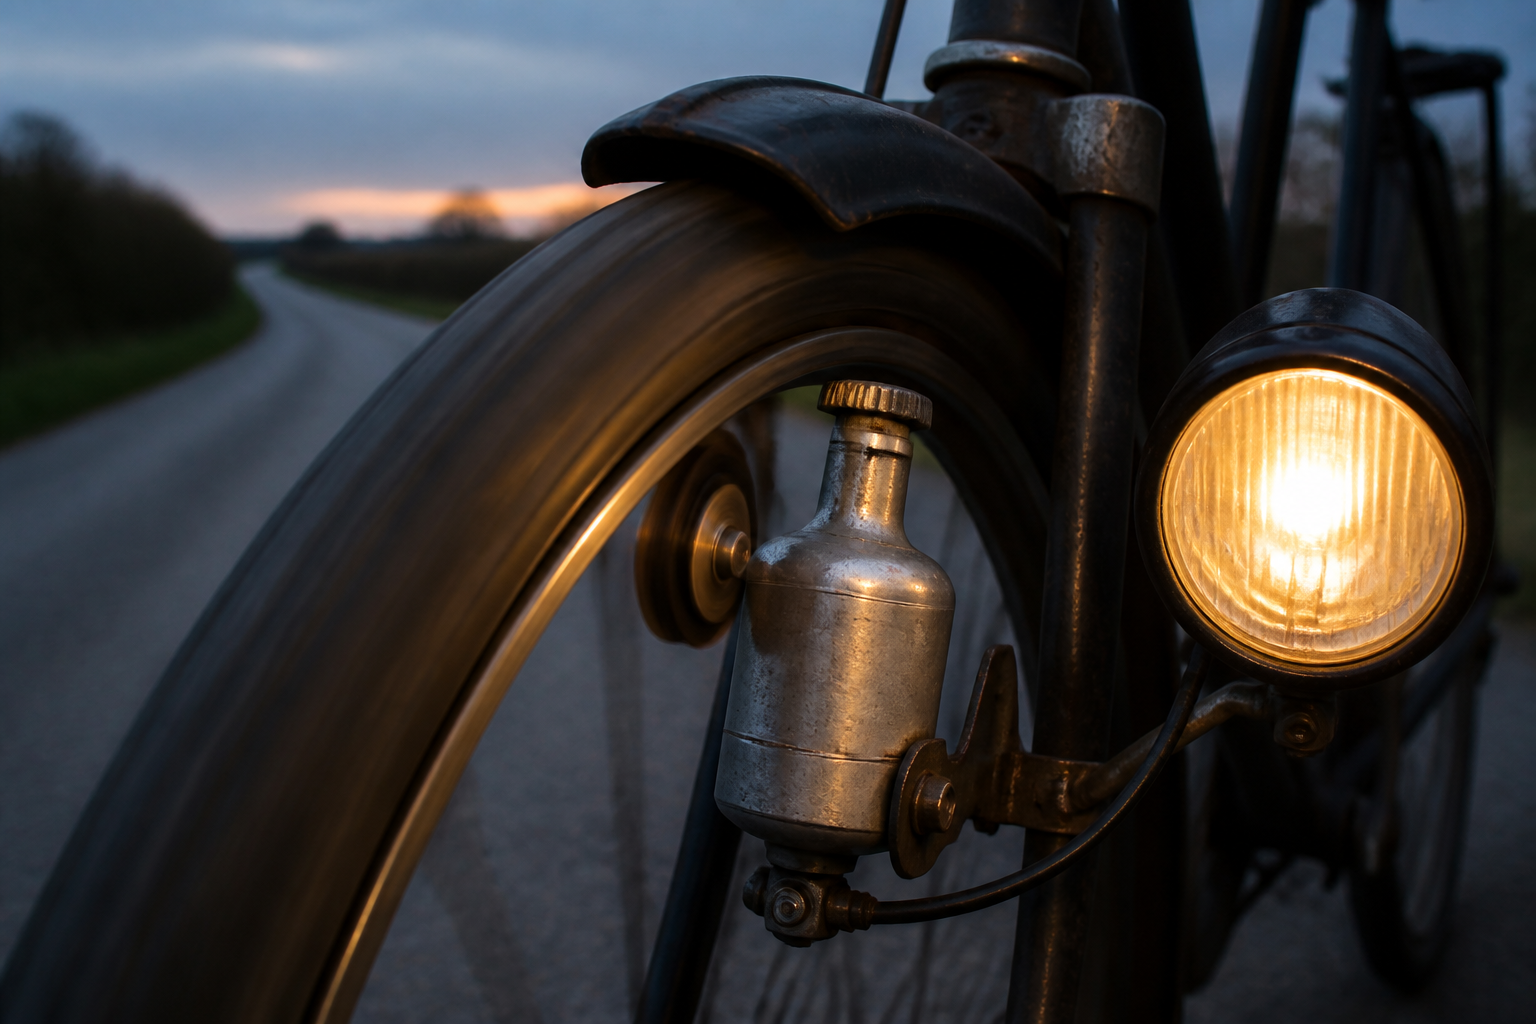
\includegraphics[width=0.58\linewidth]{images/book3/ai/b3-29-bicycle-dynamo.png}

{\small A bottle dynamo: the wheel turns a magnet inside a coil, the flux through the coil changes, and the lamp lights --- \omterm{thm:b1:induction:faraday}{Faraday's law} on a bicycle.}
\end{omfigure}

\section{Problem: The bicycle dynamo and the loudspeaker}

\begin{problem}[{Weekend problem --- two electromechanical converters
taken apart: a dynamo that regulates itself, and a loudspeaker whose
amplifier is also its brake}]
\label{pb:b1:induction:1}

\medskip
\noindent\textbf{Part I --- The bicycle dynamo.}
A coil of $N = 300$ turns and area $S = \qty{3.0}{cm^2}$ turns in a
uniform field $B = \qty{0.30}{T}$; its axle carries a roller of radius
$r = \qty{1.0}{cm}$ pressed against the tyre, so that the coil turns at
$\omega = v/r$ for a bicycle speed $v$. Coil resistance $r_c = \qty{4.0}{\ohm}$,
inductance $L = \qty{20}{mH}$; the lamp is a resistance $R = \qty{12}{\ohm}$.
\begin{enumerate}
  \item Flux through the coil and induced emf as functions of time;
        \omterm{def:b1:wave-propagation:signal}{amplitude} and frequency at $v = \qty{18}{km/h}$.
  \item Neglecting $L$ first: rms current and power in the lamp at
        \qty{18}{km/h}; is a ``\qty{6}{V}, \qty{3}{W}'' lamp comfortable?
  \item Mean mechanical power the cyclist supplies to the dynamo, and
        the corresponding force on the tyre (compare with rolling
        friction, about \qty{2}{N}).
  \item Explain with \omterm{thm:b1:induction:faraday}{Lenz's law} why the dynamo resists, and why a lamp
        that lights ``for free'' does not contradict energy conservation.
  \item Now include $L$: complex \omterm{def:b1:sinusoidal-impedance:impedance}{impedance} of the circuit; show that
        the current \omterm{def:b1:wave-propagation:signal}{amplitude} is $I = NBS\omega/\sqrt{(R + r_c)^2 + L^2\omega^2}$
        and that it saturates at high speed; its limit, and the
        speed at which it reaches $70\%$ of the limit.
  \item Without the inductance, what would the lamp receive at
        \qty{54}{km/h} downhill? With it?
  \item Current and lamp power at \qty{9}{km/h} and at \qty{36}{km/h}; comment
        on the self-regulation.
  \item Real dynamos rotate a magnet inside a fixed coil. Does the
        analysis change? What practical problem does it remove?
  \item What does the lamp do when the bicycle stops at a red light,
        and how do modern lights fix it?
\end{enumerate}

\medskip
\noindent\textbf{Part II --- The loudspeaker.}
Voice coil: wire length $\ell = \qty{5.0}{m}$ in a radial field $B =
\qty{1.0}{T}$, resistance $R = \qty{8.0}{\ohm}$, inductance $L = \qty{0.50}{mH}$;
moving mass (coil and cone) $m = \qty{10}{g}$; suspension stiffness
$k = \qty{1000}{N/m}$, mechanical damping $h = \qty{1.0}{N.s/m}$. Sinusoidal
regime, \omterm{def:b1:sinusoidal-impedance:complex}{complex amplitudes}.
\begin{enumerate}[resume]
  \item Force on the coil for a current $i$; back-emf for a speed $v$
        (derive both, with signs).
  \item Write the electrical and the mechanical equations.
  \item Eliminate $i$ and show that
        $\underline v = \dfrac{B\ell\,\underline u}{(R + jL\omega)(jm\omega + h + k/j\omega) + B^2\ell^2}$.
  \item At frequencies where $L\omega \ll R$, show that the coupling acts
        as an extra mechanical damping $B^2\ell^2/R$; value; resonance
        frequency of the cone and its \omterm{def:b1:transient-regimes:secondorder}{quality factor} with and without
        the electrical damping.
  \item The amplifier delivers $i$ of \omterm{def:b1:wave-propagation:signal}{amplitude} \qty{1.0}{A} at \qty{1}{kHz}:
        force, acceleration, displacement and velocity \omterm{def:b1:wave-propagation:signal}{amplitudes} of the
        cone (mass-controlled regime); back-emf \omterm{def:b1:wave-propagation:signal}{amplitude} compared with
        $Ri$.
  \item Same current at the resonance frequency: velocity \omterm{def:b1:wave-propagation:signal}{amplitude}
        (damping-controlled) and back-emf; comment.
  \item Electrical power at \qty{1}{kHz}; mechanical power dissipated in
        $h$ (taken as the sound and suspension losses); \omterm{def:b1:heat-engines:efficiency}{efficiency}.
  \item Why is the sound pressure proportional to the cone's
        acceleration (admit it) the reason a mass-controlled cone gives a
        flat response above resonance?
  \item Why must the field be radial, and why is a tweeter small?
  \item Sketch the modulus of the \omterm{def:b1:sinusoidal-impedance:impedance}{impedance} $\underline u/\underline i$ seen
        by the amplifier from \qty{10}{Hz} to \qty{10}{kHz}: value at low
        frequency, at resonance (use the damping-controlled velocity),
        and at \qty{10}{kHz}.
\end{enumerate}

\medskip
\noindent\textbf{Part III --- Backward, and the books.}
\begin{enumerate}[resume]
  \item The same device as a microphone: a sound moves the cone at
        $v = \qty{1.0}{mm/s}$; open-circuit \omterm{def:b1:dc-circuits:voltage}{voltage}.
  \item Loaded by $R_L = \qty{600}{\ohm}$: current, and the braking force
        on the cone; show that the microphone takes power from the sound
        through an effective damping $B^2\ell^2/(R + R_L)$.
  \item The coil is wound on an aluminium cylinder (the former), a
        closed turn of length \qty{0.10}{m} and resistance \qty{1.0}{m\ohm}:
        damping it adds; why formers are slit.
  \item Tap the cone of a loudspeaker whose terminals are left open,
        then of one whose terminals are shorted: which one rings longer,
        and why?
  \item Write the energy balance of the loudspeaker over one period at
        \omterm{def:b1:transient-regimes:firstorder}{steady state}, naming every term.
  \item Sum up: for each device, the law used and the two numbers
        worth remembering.
\end{enumerate}
\end{problem}
